% Provenance (never printed): cycle 4 SVT/physique, "La planete Terre,
% l'environnement": the movements of the atmosphere, weather and its
% forecast; see sources/book1/PROVENANCE.md. Book 1, grade 8, chapter 3.
% Vocabulary guard: owns air mass, front (warm, cold), depression (homograph:
% phrase-level linking only), anticyclone, isobar, weather forecast. The
% rotation of the winds around lows and highs is told (deflection, recalled
% from ch. g8.2); the occluded front is named in prose only; numerical models
% are told, not taught.
\chapter{Massa Udara, Front, dan Peta Cuaca}\label{ch:g8:fronts-and-weather-maps}

Pagi itu cerah dan tenang. Menjelang tengah hari, guratan-guratan putih
yang tipis muncul sangat tinggi di langit, lalu perlahan melebar menjadi
selubung pucat yang meredupkan Matahari. Pada sore hari \omterm{def:g4:clouds-rain-snow:cloud}{awan} menebal dan
turun makin rendah; menjelang malam turun \omterm{def:g4:clouds-rain-snow:precipitation}{hujan} yang tetap. Pada malam
hari udara menjadi hangat dan lembap, lalu sebuah garis \omterm{def:g4:clouds-rain-snow:cloud}{awan} yang gelap
membawa \omterm{def:g4:clouds-rain-snow:precipitation}{hujan} deras yang singkat dan embusan angin. Keesokan paginya
cerah, segar, dan berangin. Dalam dua hari, sebuah \emph{\omterm{def:g8:fronts-and-weather-maps:depression}{depresi}} telah
melintas di atas kota itu, beserta kedua \omterm{def:g8:fronts-and-weather-maps:front}{frontnya}.
% ledger: ucar:warm-front, ucar:cold-front

\begin{omfigure}
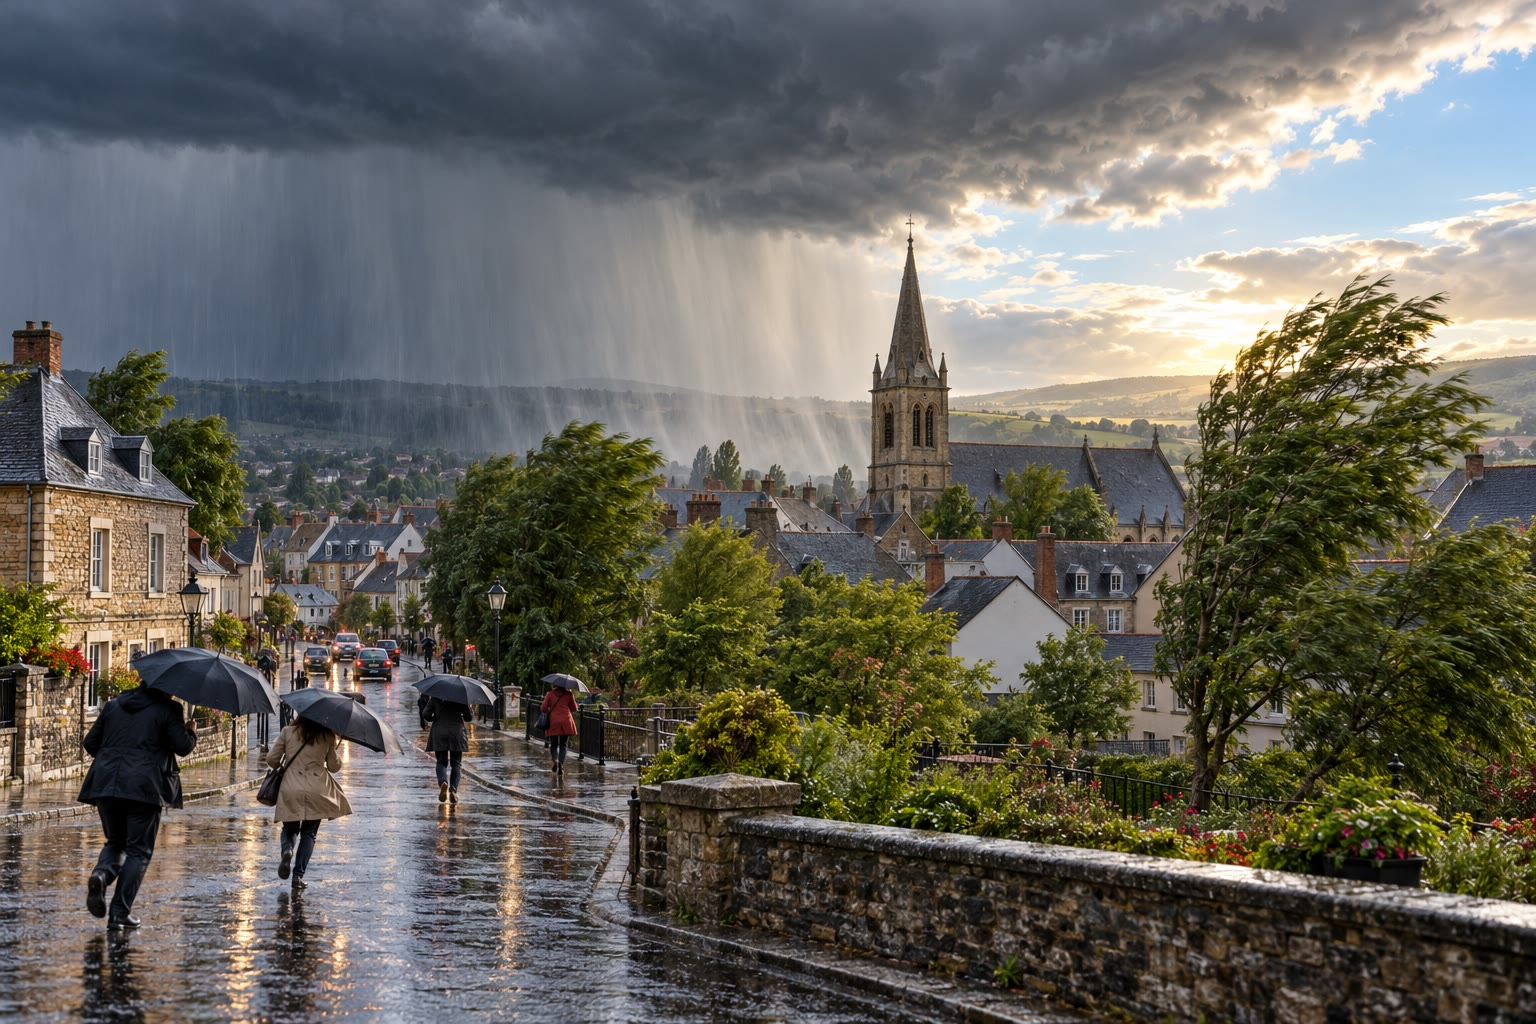
\includegraphics[width=0.6\linewidth]{images/book1/ai/g8-rain-arriving.jpg}

{\small Tirai \omterm{def:g4:clouds-rain-snow:precipitation}{hujan} tiba di atas sebuah kota di bawah dasar \omterm{def:g4:clouds-rain-snow:cloud}{awan} yang
gelap, sementara langit di belakang gereja masih cerah (ilustrasi AI dari
suatu adegan umum).}
\label{fig:g8:fronts-and-weather-maps:rain}
\end{omfigure}

Para prakirawan \omterm{def:g1:watching-the-weather:weather}{cuaca} sudah melihatnya datang beberapa hari sebelumnya.
Bab ini menunjukkan caranya: udara di langit kita datang dalam massa yang
besar, massa-massa itu bertemu di sepanjang \omterm{def:g8:fronts-and-weather-maps:front}{front}, dan \omterm{def:g2:drawing-to-map:map}{peta} tekanan
menunjukkan ke mana semuanya bergerak.

\begin{recall}
Udara menekan segala sesuatu yang disentuhnya; barometer mengukur tekanan
ini dalam hektopascal (buku-buku fisika), dan di \omterm{def:g4:world-physical-map:altitude}{permukaan laut} besarnya
sekitar \qty{1013}{hPa} (\cref{ch:g8:the-atmosphere}). \omterm{def:g4:clouds-rain-snow:cloud}{Awan} terbentuk
ketika udara lembap naik dan mendingin (\cref{ch:g4:clouds-rain-snow}). Di
permukaan tanah, angin bertiup dari tekanan tinggi ke tekanan rendah, dan
perputaran Bumi membelokkannya: ke kanan di \omterm{def:g3:continents-and-oceans:equator}{belahan bumi utara}. Di antara
sekitar \ang{30} dan \ang{60}, \omterm{def:g8:winds-global-circulation:global-winds}{angin baratan} membawa \omterm{def:g5:natural-hazards:storm}{badai} yang datang
silih berganti (\cref{ch:g8:winds-global-circulation}).
\end{recall}

\section{Massa udara}

Udara yang berhari-hari diam di atas tempat yang sama memperoleh sifat
permukaan di bawahnya. Di atas \omterm{def:g2:water-on-earth:ocean}{samudra} yang hangat, udara itu menjadi
hangat dan lembap; di atas daratan yang membeku, dingin dan kering. Ketika
bergerak pergi, udara itu membawa sifat ini bersamanya, kadang-kadang
sampai ribuan kilometer jauhnya.
% ledger: noaa:air-mass

\begin{definition}[Massa udara]\label{def:g8:fronts-and-weather-maps:air-mass}
Yang disebut \emph{massa udara}\index{massa udara} adalah tubuh udara yang
sangat besar yang suhu dan kelembapannya hampir sama di mana-mana pada
\omterm{def:g4:world-physical-map:altitude}{ketinggian} tertentu. Massa udara memperoleh sifat-sifat itu dari wilayah
tempat ia terbentuk, yaitu \emph{daerah sumbernya}.
\end{definition}
% ledger: noaa:air-mass

Para prakirawan menamai \omterm{def:g8:fronts-and-weather-maps:air-mass}{massa udara} dengan dua huruf. Huruf pertama
menyatakan tempat ia terbentuk: \emph{c} (kontinental) di atas daratan,
sehingga kering; \emph{m} (maritim) di atas \omterm{def:g2:water-on-earth:ocean}{samudra}, sehingga lembap. Huruf
kedua menyatakan seberapa dinginnya: \emph{A} (arktik) di atas wilayah
kutub, \emph{P} (polar) di atas \omterm{def:g6:latitude-longitude:latitude}{lintang} tinggi, \emph{T} (tropis) di atas
\omterm{def:g6:latitude-longitude:latitude}{lintang} rendah. Udara dari \omterm{def:g5:weather-and-climate:desert}{gurun} yang panas adalah cT, panas dan kering;
udara dari Arktik adalah cA, sangat dingin dan kering.
% ledger: noaa:air-mass

\begin{omfigure}
\begin{tikzpicture}
\begin{axis}[ommap, width=12.6cm, xmin=-100, xmax=60, ymin=10, ymax=85,
  xtick={-90,-60,...,60}, ytick={20,40,60,80},
  xticklabels={$90^\circ$BB,$60^\circ$BB,$30^\circ$BB,$0^\circ$,$30^\circ$BT,$60^\circ$BT},
  yticklabels={$20^\circ$LU,$40^\circ$LU,$60^\circ$LU,$80^\circ$LU},
  tick label style={font=\scriptsize}]
  \addplot[fill=omLithAlluv, draw=black!45, line width=0.2pt] table {figdata/out/shared-geo-land.dat};
  \tikzset{src/.style={line width=0.9pt, fill opacity=0.35, text opacity=1, font=\scriptsize, align=center}}
  \draw[src, draw=omCold, fill=omCold!35] (axis cs:-30,79) ellipse [x radius=26, y radius=4.5];
  \node[font=\scriptsize, align=center, fill=white, inner sep=1pt] at (axis cs:-30,79) {\textbf{cA}: sangat dingin, kering};
  \draw[src, draw=omCold, fill=omCold!25] (axis cs:-35,55) ellipse [x radius=14, y radius=6];
  \node[font=\scriptsize, align=center, fill=white, inner sep=1pt] at (axis cs:-35,55) {\textbf{mP}: dingin,\\ lembap};
  \draw[src, draw=omCold, fill=omCold!25] (axis cs:-84,60) ellipse [x radius=12, y radius=7];
  \node[font=\scriptsize, align=center, fill=white, inner sep=1pt] at (axis cs:-84,60) {\textbf{cP}: dingin,\\ kering};
  \draw[src, draw=omCold, fill=omCold!25] (axis cs:45,62) ellipse [x radius=14, y radius=7];
  \node[font=\scriptsize, align=center, fill=white, inner sep=1pt] at (axis cs:45,62) {\textbf{cP}: dingin,\\ kering};
  \draw[src, draw=omWarm, fill=omWarm!25] (axis cs:-45,28) ellipse [x radius=16, y radius=6];
  \node[font=\scriptsize, align=center, fill=white, inner sep=1pt] at (axis cs:-45,28) {\textbf{mT}: hangat,\\ lembap};
  \draw[src, draw=omWarm, fill=omWarm!25] (axis cs:10,24) ellipse [x radius=15, y radius=6];
  \node[font=\scriptsize, align=center, fill=white, inner sep=1pt] at (axis cs:10,24) {\textbf{cT}: panas,\\ kering};
\end{axis}
\end{tikzpicture}

{\small Daerah-daerah sumber \omterm{def:g8:fronts-and-weather-maps:air-mass}{massa udara} yang khas di sekitar Atlantik
Utara (skematis): di atas Arktik, \omterm{def:g3:continents-and-oceans:continent}{benua-benua} yang dingin, \omterm{def:g2:water-on-earth:ocean}{samudra} di
utara, \omterm{def:g2:water-on-earth:ocean}{samudra} subtropis, dan Sahara. Biru: \omterm{def:g8:fronts-and-weather-maps:air-mass}{massa udara} dingin; merah:
\omterm{def:g8:fronts-and-weather-maps:air-mass}{massa udara} hangat.}
% ledger: noaa:air-mass, data:ne-land (schematic regions)
\label{fig:g8:fronts-and-weather-maps:sources}
\end{omfigure}

\section{Front}

Ketika sebuah \omterm{def:g8:fronts-and-weather-maps:air-mass}{massa udara} bergerak, ia bertemu dengan \omterm{def:g8:fronts-and-weather-maps:air-mass}{massa udara} yang
lain. Keduanya tidak mudah bercampur: keduanya tetap terpisah, dengan
batas yang sempit di antaranya, tempat \omterm{def:g1:watching-the-weather:weather}{cuaca} berubah.
% ledger: mo:fronts, ucar:cold-front

\begin{definition}[Front]\label{def:g8:fronts-and-weather-maps:front}
Yang disebut \emph{front}\index{front} adalah batas di permukaan tanah
antara dua \omterm{def:g8:fronts-and-weather-maps:air-mass}{massa udara} yang suhu dan kelembapannya berbeda. Pada
\emph{front dingin}\index{front dingin}, udara dingin mendesak masuk ke
udara yang lebih hangat dan menggantikan tempatnya; pada \emph{front
hangat}\index{front hangat}, udara hangat mendesak masuk ke udara yang
lebih dingin dan menggantikan tempatnya.
\end{definition}
% ledger: mo:fronts, ucar:cold-front, ucar:warm-front

Udara dingin lebih rapat daripada udara hangat. Pada \omterm{def:g8:fronts-and-weather-maps:front}{front dingin}, udara
dingin menyusup ke bawah udara hangat seperti baji dan mengangkatnya
dengan tajam. Udara yang hangat dan lembap naik dengan cepat dan membentuk
\omterm{def:g4:clouds-rain-snow:cloud}{awan} yang menjulang, \omterm{def:g4:clouds-rain-snow:cloud-families}{kumulus} dan \omterm{def:g4:clouds-rain-snow:cloud-families}{kumulonimbus}: \omterm{def:g8:fronts-and-weather-maps:front}{front} ini membawa \omterm{def:g4:clouds-rain-snow:precipitation}{hujan}
deras, kadang-kadang \omterm{def:g4:clouds-rain-snow:precipitation}{hujan es} dan guntur, embusan angin, serta penurunan
suhu yang mendadak. Setelah \omterm{def:g8:fronts-and-weather-maps:front}{front} lewat, \omterm{def:g4:clouds-rain-snow:precipitation}{hujan} berhenti dan langit menjadi
cerah. \omterm{def:g8:fronts-and-weather-maps:front}{Front dingin} bergerak cepat, sampai dua kali lebih cepat daripada
\omterm{def:g8:fronts-and-weather-maps:front}{front hangat}.
% ledger: ucar:cold-front

\begin{omfigure}
\begin{tikzpicture}[font=\footnotesize, >={Stealth[length=2.2mm]}, yscale=0.7, xscale=0.95]
  % ground
  \draw[line width=0.8pt] (0,0) -- (15,0);
  % cold wedge, nose at x = 8.2
  \fill[omCold!18] (0,0) -- (0,3.4) .. controls (4.5,3.2) and (7.2,2.4) .. (7.9,0.8)
    .. controls (8.1,0.35) and (8.2,0.12) .. (8.25,0) -- cycle;
  \draw[omCold, line width=1pt] (0,3.4) .. controls (4.5,3.2) and (7.2,2.4) .. (7.9,0.8)
    .. controls (8.1,0.35) and (8.2,0.12) .. (8.25,0);
  \node[omCold, align=center] at (3.2,1.4) {\textbf{udara dingin}\\(rapat)};
  \node[omWarm, align=center] at (13.4,1.1) {\textbf{udara hangat}\\\textbf{dan lembap}};
  % cold air pushes
  \draw[->, omCold, line width=1.2pt] (4.6,0.5) -- (7.0,0.5);
  % warm air lifted
  \draw[->, omWarm, line width=1.2pt] (11.2,0.45) .. controls (9.4,0.6) and (8.6,1.4) .. (8.5,3.0);
  % cumulonimbus
  \fill[black!12] (7.3,2.6) .. controls (7.0,3.4) and (7.4,4.2) .. (7.9,4.5)
    .. controls (7.6,5.0) and (8.6,5.2) .. (9.4,5.1) -- (11.0,5.15)
    .. controls (10.6,4.9) and (10.2,4.8) .. (10.0,4.6)
    .. controls (10.4,4.0) and (10.2,3.0) .. (9.8,2.5) -- cycle;
  \draw[black!45] (7.3,2.6) .. controls (7.0,3.4) and (7.4,4.2) .. (7.9,4.5)
    .. controls (7.6,5.0) and (8.6,5.2) .. (9.4,5.1) -- (11.0,5.15)
    .. controls (10.6,4.9) and (10.2,4.8) .. (10.0,4.6)
    .. controls (10.4,4.0) and (10.2,3.0) .. (9.8,2.5) -- cycle;
  \node at (9.0,3.8) {kumulonimbus};
  \foreach \x in {7.7,8.0,...,9.6} \draw[omCold!70, line width=0.5pt] (\x,2.45) -- (\x-0.25,0.15);
  \node[anchor=west, align=left] at (9.8,1.95) {hujan deras,\\embusan angin};
  % motion
  \draw[->, line width=1.3pt] (5.7,4.3) -- (7.2,4.3);
  \node[anchor=east] at (5.6,4.3) {front bergerak};
  \node[anchor=north] at (8.25,-0.1) {front di permukaan tanah};
  \node[anchor=north west, align=left] at (0.1,-0.1) {di belakang: lebih sejuk, cerah};
  \node[anchor=north east, align=right] at (15,-0.1) {di depan: hangat, lembap};
\end{tikzpicture}

{\small \omterm{def:g8:fronts-and-weather-maps:front}{Front dingin} dilihat dari samping (\omterm{def:g4:world-physical-map:altitude}{ketinggian} sangat dibesarkan).
Udara dingin menyusup ke bawah udara hangat seperti baji; udara hangat
terangkat dengan curam dan membentuk \omterm{def:g4:clouds-rain-snow:cloud}{awan} yang menjulang.}
% ledger: ucar:cold-front
\label{fig:g8:fronts-and-weather-maps:cold}
\end{omfigure}

Pada \omterm{def:g8:fronts-and-weather-maps:front}{front hangat}, udara hangat yang ringan tidak dapat mendorong udara
dingin dari permukaan tanah: udara itu naik perlahan-lahan di atasnya,
pada lereng yang panjang dan landai. Karena itu, \omterm{def:g4:clouds-rain-snow:cloud}{awannya} muncul jauh di
depan \omterm{def:g8:fronts-and-weather-maps:front}{front}, tinggi di langit: mula-mula guratan tipis \omterm{def:g4:clouds-rain-snow:cloud}{awan} \omterm{def:g4:clouds-rain-snow:cloud-families}{sirus}, lalu
selubung sirostratus, lalu altostratus yang kelabu. Makin dekat \omterm{def:g8:fronts-and-weather-maps:front}{front} itu,
\omterm{def:g4:clouds-rain-snow:cloud}{awan} makin rendah dan tebal, dan \omterm{def:g4:clouds-rain-snow:precipitation}{hujan} yang panjang dan tetap pun mulai
turun. Setelah \omterm{def:g8:fronts-and-weather-maps:front}{front} lewat, udara lebih hangat dan lebih lembap.
% ledger: ucar:warm-front, bom:isobars (warm front: steady rain, grey skies)

\begin{omfigure}
\begin{tikzpicture}[font=\footnotesize, >={Stealth[length=2.2mm]}]
  \draw[line width=0.8pt] (0,0) -- (15,0);
  % cold air ahead (right), warm air climbing a gentle slope from the front at x = 2.2
  \fill[omCold!18] (2.2,0) .. controls (6,0.9) and (10,2.2) .. (15,3.4) -- (15,0) -- cycle;
  \draw[omCold, line width=1pt] (2.2,0) .. controls (6,0.9) and (10,2.2) .. (15,3.4);
  \node[omCold, align=center] at (11.8,0.75) {\textbf{udara dingin}};
  \node[omWarm, align=center] at (1.4,1.6) {\textbf{udara hangat}\\\textbf{dan lembap}};
  \draw[->, omWarm, line width=1.2pt] (1.0,0.45) .. controls (4.5,0.9) and (8.5,2.4) .. (12.4,3.4);
  % clouds: nimbostratus near the front, altostratus, cirrostratus, cirrus far ahead
  \fill[black!18] (2.4,0.7) .. controls (3.2,1.8) and (5.5,2.3) .. (6.6,2.4) -- (6.4,1.25) .. controls (5,1.0) and (3.8,0.7) .. cycle;
  \node at (5.4,1.62) {nimbostratus};
  \foreach \x in {3.0,3.3,...,5.7} \draw[omCold!70, line width=0.5pt] (\x,0.95) -- (\x-0.2,0.25);
  \fill[black!10, rounded corners=4pt] (6.4,2.65) rectangle (10.0,3.25);
  \node at (8.2,2.95) {altostratus};
  \fill[black!6, rounded corners=4pt] (9.6,3.75) rectangle (12.6,4.15);
  \node at (11.1,3.95) {sirostratus};
  \foreach \x in {12.6,13.2,13.8} \draw[black!35, line width=0.6pt] (\x,4.55) .. controls (\x+0.2,4.75) and (\x+0.4,4.6) .. (\x+0.55,4.85);
  \node[anchor=south] at (13.4,4.9) {sirus};
  \draw[->, line width=1.3pt] (2.6,4.3) -- (4.1,4.3);
  \node[anchor=east] at (2.5,4.3) {front bergerak};
  \node[anchor=north] at (2.2,-0.1) {front di permukaan tanah};
  \node[anchor=north east] at (15,-0.1) {jauh di depan: awan tinggi yang pertama};
\end{tikzpicture}

{\small \omterm{def:g8:fronts-and-weather-maps:front}{Front hangat} dilihat dari samping (\omterm{def:g4:world-physical-map:altitude}{ketinggian} sangat dibesarkan).
Udara hangat naik perlahan-lahan di atas udara dingin; \omterm{def:g4:clouds-rain-snow:cloud}{awannya} makin
rendah dan tebal ketika \omterm{def:g8:fronts-and-weather-maps:front}{front} mendekat, dan \omterm{def:g4:clouds-rain-snow:precipitation}{hujannya} panjang dan tetap.}
% ledger: ucar:warm-front
\label{fig:g8:fronts-and-weather-maps:warm}
\end{omfigure}

Pada \omterm{def:g2:drawing-to-map:map}{peta} \omterm{def:g1:watching-the-weather:weather}{cuaca}, \omterm{def:g8:fronts-and-weather-maps:front}{front dingin} digambar sebagai garis biru bersegitiga, dan
\omterm{def:g8:fronts-and-weather-maps:front}{front hangat} sebagai garis merah berhiaskan setengah lingkaran.
Lambang-lambang itu terletak di sisi ke arah mana \omterm{def:g8:fronts-and-weather-maps:front}{front} bergerak. Ketika
\omterm{def:g8:fronts-and-weather-maps:front}{front dingin} yang cepat menyusul \omterm{def:g8:fronts-and-weather-maps:front}{front hangat}, keduanya bergabung menjadi
\emph{\omterm{def:g8:fronts-and-weather-maps:front}{front} oklusi}, yang digambar dengan warna ungu dan memuat kedua
lambang itu.
% ledger: mo:fronts, ucar:cold-front

\section{Depresi dan antisiklon}

\omterm{def:g8:fronts-and-weather-maps:front}{Front} lahir di dalam pusaran udara raksasa yang melintasi \omterm{def:g6:latitude-longitude:latitude}{lintang} tengah.
Di tempat udara naik, tekanan di permukaan tanah lebih rendah daripada di
sekelilingnya; di tempat udara turun, tekanannya lebih tinggi.
% ledger: bom:highs-lows

\begin{definition}[Depresi dan antisiklon]\label{def:g8:fronts-and-weather-maps:depression}
Yang disebut \emph{depresi}\index{depresi (cuaca)}, atau daerah tekanan
rendah, adalah wilayah yang tekanannya di \omterm{def:g4:world-physical-map:altitude}{permukaan laut} lebih rendah
daripada di sekelilingnya. Yang disebut \emph{antisiklon}\index{antisiklon},
atau daerah tekanan tinggi, adalah wilayah yang tekanannya lebih tinggi
daripada di sekelilingnya.
\end{definition}
% ledger: bom:isobars, bom:highs-lows
\phantomsection\label{def:g8:fronts-and-weather-maps:anticyclone}

Angin bertiup dari daerah tekanan tinggi ke daerah tekanan rendah, tetapi
perputaran Bumi membelokkannya, sehingga akhirnya angin bertiup hampir
mengelilingi pusat-pusatnya. Di \omterm{def:g3:continents-and-oceans:equator}{belahan bumi utara}, angin berputar
berlawanan arah jarum jam di sekitar \omterm{def:g8:fronts-and-weather-maps:depression}{depresi} dan searah jarum jam di
sekitar \omterm{def:g8:fronts-and-weather-maps:depression}{antisiklon}; di \omterm{def:g3:continents-and-oceans:equator}{belahan bumi selatan}, sebaliknya. Di dalam \omterm{def:g8:fronts-and-weather-maps:depression}{depresi},
udara mengalir masuk di dekat tanah, naik, mendingin, dan membentuk \omterm{def:g4:clouds-rain-snow:cloud}{awan}:
\omterm{def:g8:fronts-and-weather-maps:depression}{depresi} membawa \omterm{def:g4:clouds-rain-snow:cloud}{awan}, \omterm{def:g4:clouds-rain-snow:precipitation}{hujan}, dan angin, beserta \omterm{def:g8:fronts-and-weather-maps:front}{front-frontnya}. Di dalam
\omterm{def:g8:fronts-and-weather-maps:depression}{antisiklon}, udara turun dan menghangat selama turun: \omterm{def:g8:fronts-and-weather-maps:depression}{antisiklon} membawa
\omterm{def:g1:watching-the-weather:weather}{cuaca} yang kering dan tenang dengan angin yang lemah. \omterm{def:g8:fronts-and-weather-maps:depression}{Antisiklon} yang khas
mempunyai tekanan sekitar \qty{1020}{hPa} atau lebih di pusatnya; \omterm{def:g8:fronts-and-weather-maps:depression}{depresi}
yang dalam turun di bawah \qty{980}{hPa}.
% ledger: bom:highs-lows, bom:isobars, mo:global-circ

\begin{omfigure}
\begin{minipage}[c]{0.36\linewidth}\centering
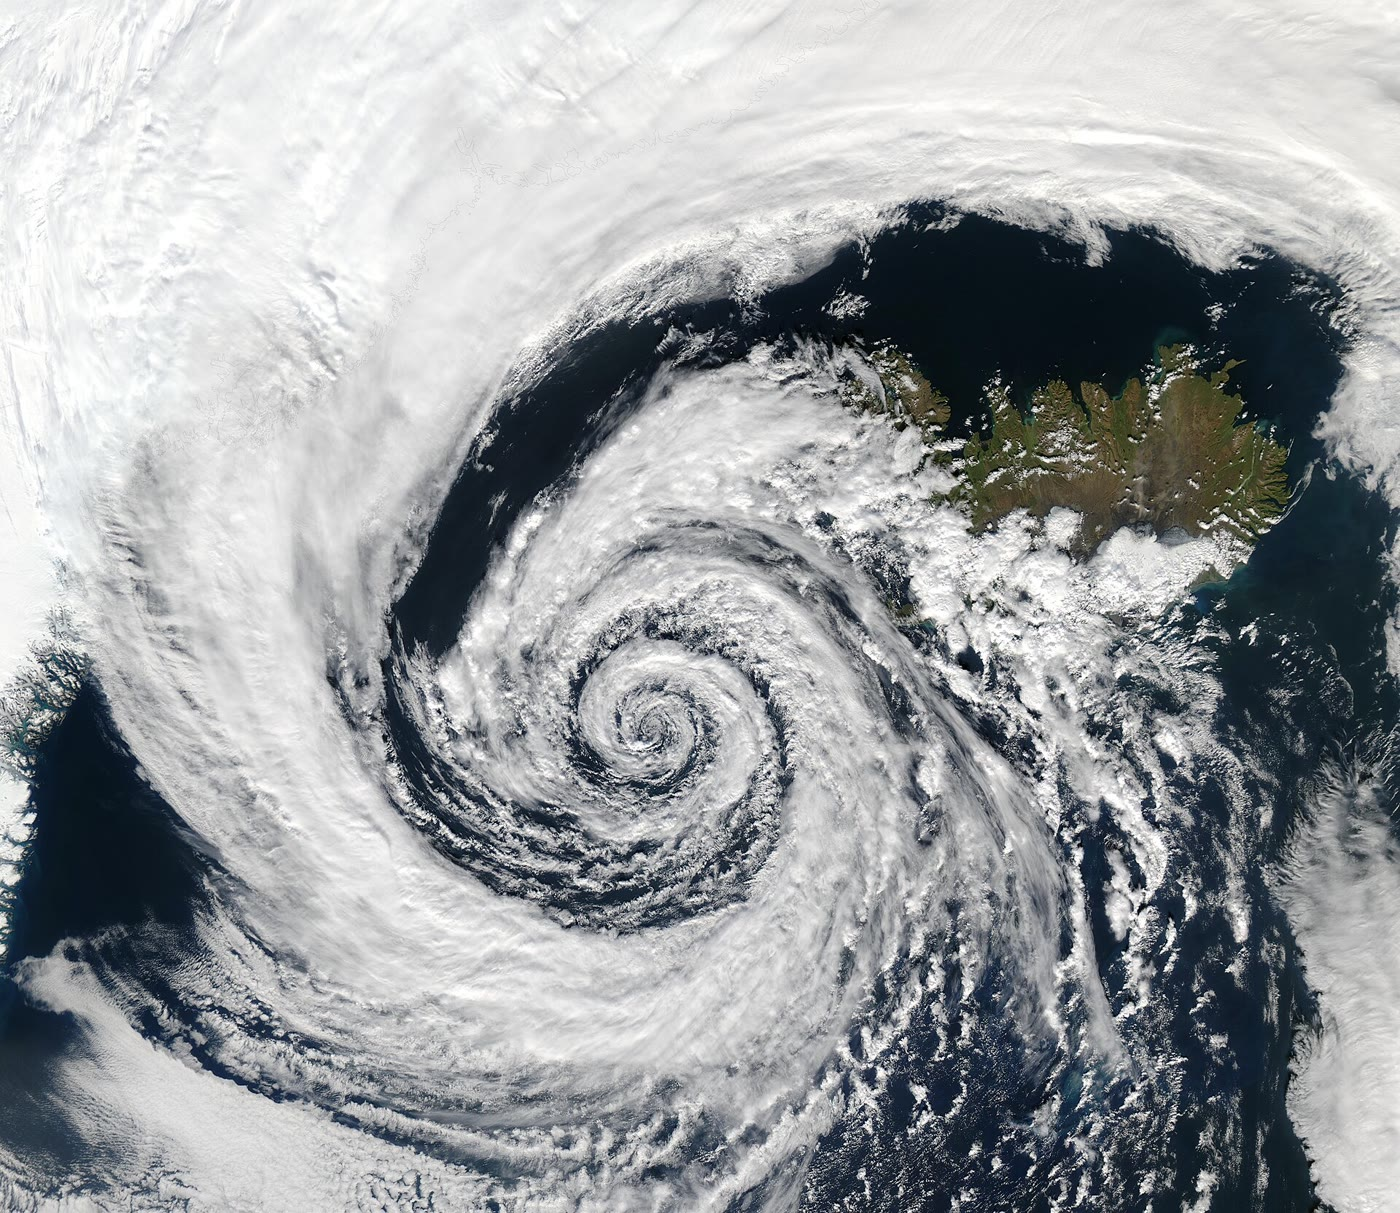
\includegraphics[width=\linewidth]{images/book1/g8-iceland-low.jpg}
\end{minipage}\hfill
\begin{minipage}[c]{0.6\linewidth}\raggedright
{\small Sebuah \omterm{def:g8:fronts-and-weather-maps:depression}{depresi} di barat daya Islandia (pulau di kanan atas)
yang dipotret satelit Aqua milik NASA pada 4~September 2003. \omterm{def:g4:clouds-rain-snow:cloud}{Awannya}
berpilin masuk ke arah pusat, berputar berlawanan arah jarum jam seperti
pada setiap \omterm{def:g8:fronts-and-weather-maps:depression}{depresi} di \omterm{def:g3:continents-and-oceans:equator}{belahan bumi utara}. NASA/GSFC, MODIS Rapid Response
Team, Jacques Descloitres (domain publik, melalui Wikimedia Commons).}
\end{minipage}
% ledger: commons:iceland-low, bom:highs-lows
\label{fig:g8:fronts-and-weather-maps:iceland}
\end{omfigure}

\section{Isobar dan peta cuaca}

Untuk melihat \omterm{def:g8:fronts-and-weather-maps:depression}{depresi} dan \omterm{def:g8:fronts-and-weather-maps:depression}{antisiklon}, para prakirawan menggambar \omterm{def:g2:drawing-to-map:map}{peta}
tekanan. Setiap stasiun mengukur tekanannya dan mengoreksinya ke \omterm{def:g4:world-physical-map:altitude}{permukaan
laut}, sehingga stasiun di puncak \omterm{def:g1:landscapes-around-us:landform}{gunung} dapat dibandingkan dengan stasiun
di pantai. Lalu digambarlah garis-garis yang melalui semua tempat yang
tekanannya sama.
% ledger: bom:isobars

\begin{definition}[Isobar]\label{def:g8:fronts-and-weather-maps:isobar}
Yang disebut \emph{isobar}\index{isobar} adalah garis pada \omterm{def:g2:drawing-to-map:map}{peta} yang
menghubungkan tempat-tempat yang tekanannya di \omterm{def:g4:world-physical-map:altitude}{permukaan laut} sama. Isobar
diberi angka dalam hektopascal dan sering digambar setiap \qty{4}{hPa}.
\end{definition}
% ledger: bom:isobars (the 4 hPa step is the one of this book's maps)

Di sekitar \omterm{def:g8:fronts-and-weather-maps:depression}{depresi}, \omterm{def:g8:fronts-and-weather-maps:isobar}{isobar} membentuk lingkaran-lingkaran tertutup, dengan
tekanan terendah di pusatnya, yang ditandai R; di sekitar \omterm{def:g8:fronts-and-weather-maps:depression}{antisiklon},
\omterm{def:g8:fronts-and-weather-maps:isobar}{isobar} membentuk lingkaran dengan tekanan tertinggi di pusatnya, yang
ditandai T. Di tempat \omterm{def:g8:fronts-and-weather-maps:isobar}{isobar-isobar} saling berdekatan, tekanan berubah
dengan cepat dari satu tempat ke tempat berikutnya, dan anginnya kencang;
di tempat \omterm{def:g8:fronts-and-weather-maps:isobar}{isobar-isobar} berjauhan, anginnya lemah.
% ledger: bom:isobars

\begin{omfigure}
\begin{tikzpicture}
\begin{axis}[width=14cm, axis equal image, xmin=0, xmax=2400, ymin=0, ymax=1600,
  hide axis, clip=true, axis background/.style={fill=white}]
  \addplot[isobar] table {figdata/out/grade-8-weather_map-isobars.dat};
  \addplot[warm front] table {figdata/out/grade-8-weather_map-warm.dat};
  \addplot[cold front] table {figdata/out/grade-8-weather_map-cold.dat};
  \addplot[quiver={u=\thisrow{u}, v=\thisrow{v}}, -{Stealth[length=1.5mm]}, omMeth, line width=0.6pt]
    table[x=x, y=y] {figdata/out/grade-8-weather_map-winds.dat};
  \addplot[only marks, mark=none, nodes near coords, point meta=explicit symbolic,
    every node near coord/.style={anchor=center, font=\tiny, fill=white, inner sep=0.6pt}]
    table[x=x, y=y, meta=level] {figdata/out/grade-8-weather_map-labels.dat};
  \node[font=\Large\bfseries, omCold, fill=white, inner sep=1pt] at (axis cs:690,1010) {R};
  \node[font=\scriptsize, anchor=north, fill=white, inner sep=0.5pt] at (axis cs:690,968) {980};
  \node[font=\Large\bfseries, omWarm] at (axis cs:1950,520) {T};
  \node[font=\scriptsize, anchor=north] at (axis cs:1950,485) {1034};
  \addplot[only marks, mark=square*, mark size=2pt, black] table[x=x, y=y] {figdata/out/grade-8-weather_map-town.dat};
  \node[font=\footnotesize\bfseries, anchor=west, fill=white, inner sep=1pt] at (axis cs:870,380) {K};
  \fill[white] (axis cs:1930,1450) rectangle (axis cs:2290,1585);
  \draw[line width=1pt] (axis cs:1950,1480) -- (axis cs:2250,1480);
  \pgfplotsinvokeforeach{1950,2050,2150,2250}{\draw (axis cs:#1,1460) -- (axis cs:#1,1500);}
  \node[font=\scriptsize, anchor=south] at (axis cs:2100,1495) {300 km};
\end{axis}
\end{tikzpicture}

{\small \omterm{def:g2:drawing-to-map:map}{Peta} \omterm{def:g1:watching-the-weather:weather}{cuaca} sebuah hari khayalan di \omterm{def:g3:continents-and-oceans:equator}{belahan bumi utara}, yang
dihitung dari sebuah model tekanan. \omterm{def:g8:fronts-and-weather-maps:isobar}{Isobar} setiap \qty{4}{hPa}; \omterm{def:g8:fronts-and-weather-maps:depression}{depresi} R
(\qty{980}{hPa}) membawa sebuah \omterm{def:g8:fronts-and-weather-maps:front}{front hangat} (merah) dan sebuah \omterm{def:g8:fronts-and-weather-maps:front}{front
dingin} (biru); \omterm{def:g8:fronts-and-weather-maps:depression}{antisiklon} T (\qty{1034}{hPa}) terletak di sebelah timur.
T dan R: tekanan tinggi dan tekanan rendah. Panah hijau: angin, lebih
panjang di tempat angin lebih kencang. K: kota dalam soal.}
% ledger: bom:isobars, bom:highs-lows, mo:fronts (figdata/grade-8/weather_map.py)
\label{fig:g8:fronts-and-weather-maps:map}
\end{omfigure}

\begin{method}[Membaca peta cuaca]
\begin{enumerate}
  \item Temukan pusat-pusatnya: R untuk \omterm{def:g8:fronts-and-weather-maps:depression}{depresi}, T untuk \omterm{def:g8:fronts-and-weather-maps:depression}{antisiklon},
        beserta tekanannya.
  \item Bacalah \omterm{def:g8:fronts-and-weather-maps:isobar}{isobarnya}: nilainya naik ke arah T dan turun ke arah R.
        \omterm{def:g8:fronts-and-weather-maps:isobar}{Isobar} yang berdekatan berarti angin yang kencang.
  \item Temukan arah angin: di \omterm{def:g3:continents-and-oceans:equator}{belahan bumi utara}, angin bertiup hampir
        sejajar dengan \omterm{def:g8:fronts-and-weather-maps:isobar}{isobar}, dengan tekanan rendah di sebelah kirinya,
        sedikit membelok ke arah tekanan rendah.
  \item Temukan \omterm{def:g8:fronts-and-weather-maps:front}{front-frontnya} dan arah geraknya (sisi lambang-lambangnya),
        lalu udara di kedua sisinya: apa yang akan datang berikutnya?
\end{enumerate}
\end{method}
% ledger: bom:isobars, bom:highs-lows, mo:fronts

\begin{example}[Cuaca di kota K]
Pada \omterm{def:g2:drawing-to-map:map}{peta}, K terletak di selatan \omterm{def:g8:fronts-and-weather-maps:front}{front hangat} dan di timur \omterm{def:g8:fronts-and-weather-maps:front}{front dingin}:
di dalam udara hangat di antara kedua \omterm{def:g8:fronts-and-weather-maps:front}{front}. \omterm{def:g8:fronts-and-weather-maps:front}{Front hangat} sudah
melewatinya. Di sana \omterm{def:g8:fronts-and-weather-maps:isobar}{isobar-isobar} membentang dari barat daya ke timur
laut, dengan tekanan rendah di barat laut: angin bertiup dari barat daya,
hangat dan lembap. \omterm{def:g8:fronts-and-weather-maps:front}{Front dingin} datang dari barat. Segitiga-segitiganya
menghadap ke timur, ke arah kota: dalam beberapa jam akan datang \omterm{def:g4:clouds-rain-snow:precipitation}{hujan}
deras yang singkat dan embusan angin, lalu angin akan berbalik dari barat
atau barat laut, udara akan menjadi lebih sejuk, dan langit akan cerah.
\end{example}
% ledger: ucar:cold-front (figdata/grade-8/weather_map.py: wind at T from 227 degrees)

Barometer memberi peringatannya sendiri, bahkan tanpa \omterm{def:g2:drawing-to-map:map}{peta}. Misalkan
seluruh \omterm{def:g2:drawing-to-map:map}{peta} di atas bergeser ke timur, tanpa berubah, dengan kecepatan
\qty{40}{km} per jam, dan sebuah barometer perekam berdiri di stasiun S,
di sebelah timur \omterm{def:g8:fronts-and-weather-maps:front}{front-front} itu. Selama dua setengah hari, barometer itu
akan menggambar rekaman di bawah ini.

\begin{omfigure}
\begin{tikzpicture}
\begin{axis}[width=0.86\linewidth, height=5.4cm, xmin=0, xmax=60, ymin=980, ymax=1040,
  xtick={0,12,...,60}, ytick={980,990,...,1040},
  xlabel={jam sejak awal rekaman}, ylabel={tekanan (hPa)},
  axis x line=bottom, axis y line=left, axis line style={-},
  grid=major, grid style={black!10},
  tick label style={font=\scriptsize}, label style={font=\small}, clip=false]
  \draw[omWarm!80!black, dashed] (axis cs:26.28,980) -- (axis cs:26.28,1040);
  \draw[omCold!80!black, dashed] (axis cs:38.49,980) -- (axis cs:38.49,1040);
  \node[font=\scriptsize, omWarm!80!black, anchor=south, fill=white, inner sep=1pt] at (axis cs:26.28,1032) {front hangat};
  \node[font=\scriptsize, omCold!80!black, anchor=south, fill=white, inner sep=1pt] at (axis cs:38.49,1032) {front dingin};
  \addplot[black!80, line width=1pt] table[x=hour, y=p_hPa] {figdata/out/grade-8-barogram-trace.dat};
  \node[font=\scriptsize, anchor=north west, align=left] at (axis cs:2,1028) {antisiklon:\\cuaca tenang};
  \node[font=\scriptsize, anchor=west] at (axis cs:39.5,986) {terendah};
\end{axis}
\end{tikzpicture}

{\small Rekaman barometer di stasiun S selagi \omterm{def:g2:drawing-to-map:map}{peta} di atas bergeser ke
timur dengan kecepatan \qty{40}{km} per jam (situasi rekaan, dihitung dari
medan tekanan \omterm{def:g2:drawing-to-map:map}{peta} itu). Garis putus-putus: \omterm{def:g8:fronts-and-weather-maps:front}{front hangat} dan \omterm{def:g8:fronts-and-weather-maps:front}{front dingin}
yang melewati stasiun.}
% ledger: (invented region: weather situation of figdata/grade-8/weather_map.py, record from figdata/grade-8/barogram.py)
\end{omfigure}

\begin{example}[Membaca rekaman barometer]\label{ex:g8:fronts-and-weather-maps:barogram}
Selama 8 jam pertama tekanan naik sampai sekitar \qty{1031}{hPa}:
\omterm{def:g8:fronts-and-weather-maps:depression}{antisiklon} melintas di atas S, dengan \omterm{def:g1:watching-the-weather:weather}{cuaca} yang tenang. Lalu tekanan turun
selama 30 jam, sebesar sekitar \qty{45}{hPa}: \omterm{def:g8:fronts-and-weather-maps:depression}{depresi} sedang datang.
Tekanan turun paling cepat beberapa jam sebelum \omterm{def:g8:fronts-and-weather-maps:front}{front hangat} lewat, lebih
lambat di dalam udara hangat di belakangnya, dan mencapai titik
terendahnya, sekitar \qty{986}{hPa}, tepat ketika \omterm{def:g8:fronts-and-weather-maps:front}{front dingin} lewat. Lalu
tekanan naik: \omterm{def:g8:fronts-and-weather-maps:depression}{depresi} sedang menjauh, dan udara yang lebih sejuk dan
lebih cerah di belakang \omterm{def:g8:fronts-and-weather-maps:front}{front dingin} tiba.
% ledger: (invented region: figdata/grade-8/barogram.py), bom:highs-lows
\end{example}

\section{Bagaimana prakiraan cuaca dibuat}

\begin{definition}[Prakiraan cuaca]\label{def:g8:fronts-and-weather-maps:forecast}
Yang disebut \emph{prakiraan cuaca}\index{prakiraan cuaca} adalah
pernyataan tentang \omterm{def:g1:watching-the-weather:weather}{cuaca} yang diharapkan di suatu tempat dalam beberapa
jam atau hari mendatang, yang disusun dari pengamatan atmosfer dan dari
hukum-hukum fisika.
\end{definition}
% ledger: mo:how-forecasts

\omterm{def:g8:fronts-and-weather-maps:forecast}{Prakiraan cuaca} dibuat dalam tiga langkah. Pertama, dinas-dinas \omterm{def:g1:watching-the-weather:weather}{cuaca} di
seluruh dunia melakukan jutaan pengamatan setiap hari: suhu, curah \omterm{def:g4:clouds-rain-snow:precipitation}{hujan},
tekanan, angin, dan kelembapan, yang diukur di stasiun darat, di \omterm{def:g2:water-on-earth:ocean}{laut},
dengan balon \omterm{def:g1:watching-the-weather:weather}{cuaca}, dengan radar, dan dari satelit. Kemudian
pengamatan-pengamatan ini dimasukkan ke dalam model komputer: komputer
yang sangat kuat menghitung, langkah demi langkah, bagaimana atmosfer akan
berubah dari keadaannya sekarang. Akhirnya, para prakirawan membaca
hasilnya, membandingkannya dengan apa yang mereka ketahui tentang wilayah
mereka, lalu menulis prakiraannya.
% ledger: mo:how-forecasts

\begin{history}[Prakiraan cuaca publik yang pertama]
Pada tahun 1854, seorang perwira angkatan \omterm{def:g2:water-on-earth:ocean}{laut}, Robert FitzRoy, diangkat
menjadi kepala sebuah kantor \omterm{def:g1:watching-the-weather:weather}{cuaca} baru di London. Setiap pagi pukul
09.00, stasiun-stasiun di sepanjang pantai mengukur \omterm{def:g1:watching-the-weather:weather}{cuaca} dan mengirimkan
hasilnya ke London lewat telegraf, penemuan terbaru pada masa itu. Pada
tahun 1859, sebuah \omterm{def:g5:natural-hazards:storm}{badai} dahsyat, \omterm{def:g5:natural-hazards:storm}{badai} \emph{Royal Charter},
menenggelamkan banyak kapal; FitzRoy lalu mendirikan layanan peringatan
\omterm{def:g5:natural-hazards:storm}{badai} bagi para pelaut, yang dimulai pada bulan Februari 1861. Pada
1~Agustus 1861 ia melangkah lebih jauh dan menerbitkan \omterm{def:g8:fronts-and-weather-maps:forecast}{prakiraan cuaca}
publik yang pertama di sebuah surat kabar, \emph{The Times}.
Prakiraan-prakiraannya melihat satu atau dua hari ke depan dan sangat
umum; prakiraan-prakiraan itulah awal dari \omterm{def:g8:fronts-and-weather-maps:forecast}{prakiraan cuaca} yang kita baca
sekarang.
\end{history}
% ledger: mo:fitzroy

\omterm{def:g8:fronts-and-weather-maps:forecast}{Prakiraan cuaca} sudah menjadi jauh lebih baik. Selama beberapa dasawarsa
terakhir, para prakirawan memperoleh kira-kira satu hari tambahan
prakiraan yang baik setiap sepuluh tahun: prakiraan untuk empat hari ke
depan sekarang sama baiknya dengan prakiraan untuk satu hari ke depan tiga
puluh tahun yang lalu. Namun, makin jauh ke depan sebuah prakiraan
melihat, makin tidak pasti prakiraan itu, karena kesalahan-kesalahan kecil
dalam pengamatan awal membesar selagi komputer melangkah maju dalam
waktu.
% ledger: bauer:day-per-decade, mo:accuracy

\begin{inthefield}[Mengamati datangnya front]
Pada hari ketika \omterm{def:g8:fronts-and-weather-maps:forecast}{prakiraan cuaca} mengumumkan datangnya sebuah \omterm{def:g8:fronts-and-weather-maps:front}{front},
amati langit setiap beberapa jam dan catat waktunya, \omterm{def:g4:clouds-rain-snow:cloud}{awannya}, anginnya,
dan suhunya. Sebelum \omterm{def:g8:fronts-and-weather-maps:front}{front hangat}, apakah guratan tinggi \omterm{def:g4:clouds-rain-snow:cloud}{awan} \omterm{def:g4:clouds-rain-snow:cloud-families}{sirus}
datang lebih dulu? Ketika \omterm{def:g8:fronts-and-weather-maps:front}{front dingin} lewat, apakah suhu turun dan angin
berubah arah? Bandingkan catatanmu dengan \omterm{def:g2:drawing-to-map:map}{peta} \omterm{def:g1:watching-the-weather:weather}{cuaca} hari itu.
\end{inthefield}

\section{Latihan}

\begin{exercise}[$\star$]\label{exo:g8:fronts-and-weather-maps:1}
Berikan arti setiap pasangan huruf dan katakan apakah \omterm{def:g8:fronts-and-weather-maps:air-mass}{massa udaranya}
hangat atau dingin, lembap atau kering: (a) mT; (b) cP; (c) cT; (d) mP.
\end{exercise}

\begin{exercise}[$\star$]\label{exo:g8:fronts-and-weather-maps:2}
Pasangkan setiap tanda pada \omterm{def:g2:drawing-to-map:map}{peta} \omterm{def:g1:watching-the-weather:weather}{cuaca} dengan artinya: garis biru
bersegitiga; garis merah berhiaskan setengah lingkaran; garis yang
menghubungkan tempat-tempat yang tekanannya sama; huruf T; huruf R.
\end{exercise}

\begin{exercise}[$\star$]\label{exo:g8:fronts-and-weather-maps:3}
Benar atau salah? Perbaiki kalimat yang salah. (a) \omterm{def:g8:fronts-and-weather-maps:depression}{Antisiklon} biasanya
membawa \omterm{def:g1:watching-the-weather:weather}{cuaca} yang tenang. (b) \omterm{def:g4:clouds-rain-snow:cloud}{Awan} \omterm{def:g8:fronts-and-weather-maps:front}{front hangat} datang sesudah \omterm{def:g8:fronts-and-weather-maps:front}{frontnya}.
(c) \omterm{def:g8:fronts-and-weather-maps:isobar}{Isobar} yang berdekatan berarti angin yang lemah. (d) Udara dingin
lebih rapat daripada udara hangat.
\end{exercise}

\begin{exercise}[$\star$]\label{exo:g8:fronts-and-weather-maps:4}
Pada \omterm{def:g2:drawing-to-map:map}{peta} \omterm{def:g1:watching-the-weather:weather}{cuaca} bab ini: (a) berapa tekanan di pusat \omterm{def:g8:fronts-and-weather-maps:depression}{depresi}? (b) Di pusat
\omterm{def:g8:fronts-and-weather-maps:depression}{antisiklon}? (c) Berapa hektopascal selisih antara dua \omterm{def:g8:fronts-and-weather-maps:isobar}{isobar} yang
bersebelahan? (d) Berapa hektopascal selisih tekanan antara kedua pusat
itu?
\end{exercise}

\begin{exercise}[$\star\star$]\label{exo:g8:fronts-and-weather-maps:5}
Urutkan peristiwa-peristiwa ini sesuai urutan terjadinya ketika sebuah
\omterm{def:g8:fronts-and-weather-maps:front}{front hangat} mendekat lalu lewat: \omterm{def:g4:clouds-rain-snow:precipitation}{hujan} yang tetap; guratan tipis \omterm{def:g4:clouds-rain-snow:cloud}{awan}
\omterm{def:g4:clouds-rain-snow:cloud-families}{sirus}; selubung kelabu altostratus; udara yang lebih hangat dan lebih
lembap; \omterm{def:g4:clouds-rain-snow:cloud}{awan} yang makin rendah dan tebal.
\end{exercise}

\begin{exercise}[$\star\star$]\label{exo:g8:fronts-and-weather-maps:6}
Jelaskan mengapa \omterm{def:g4:clouds-rain-snow:cloud}{awan} \omterm{def:g8:fronts-and-weather-maps:front}{front dingin} menjulang tinggi, sedangkan \omterm{def:g4:clouds-rain-snow:cloud}{awan} \omterm{def:g8:fronts-and-weather-maps:front}{front
hangat} menyebar berlapis-lapis. Gunakan kata-kata \emph{baji},
\emph{curam}, \emph{lereng landai}.
\end{exercise}

\begin{exercise}[$\star\star$]\label{exo:g8:fronts-and-weather-maps:7}
Pada \omterm{def:g2:drawing-to-map:map}{peta} \omterm{def:g1:watching-the-weather:weather}{cuaca}: (a) di mana angin paling kencang, di dekat R atau di
dekat T? Bagaimana kamu mengetahuinya? (b) Di utara R, dari arah mana
angin bertiup? (c) Di selatan T? (d) Apakah angin berputar searah atau
berlawanan arah jarum jam di sekitar R?
\end{exercise}

\begin{exercise}[$\star\star$]\label{exo:g8:fronts-and-weather-maps:8}
Sebuah barometer di sebuah kota menunjukkan \qty{1016}{hPa} pada pukul
06.00, \qty{1009}{hPa} pada pukul 12.00, dan \qty{1003}{hPa} pada pukul
18.00. (a) Berapa besar penurunan tekanan dalam 12 jam? (b) Apa yang
sedang datang ke arah kota itu, \omterm{def:g8:fronts-and-weather-maps:depression}{depresi} atau \omterm{def:g8:fronts-and-weather-maps:depression}{antisiklon}? (c) \omterm{def:g1:watching-the-weather:weather}{Cuaca} apa
yang dapat diperkirakan kota itu?
\end{exercise}

\begin{exercise}[$\star\star$]\label{exo:g8:fronts-and-weather-maps:9}
Udara yang sudah seminggu diam di atas Sahara bergerak ke utara melintasi
\omterm{def:g2:water-on-earth:ocean}{Laut} Tengah. (a) Namai \omterm{def:g8:fronts-and-weather-maps:air-mass}{massa udara} ini dengan kedua hurufnya. (b) Apakah
udara itu panas atau dingin, lembap atau kering, ketika berangkat? (c) Apa
yang dapat berubah pada sifatnya selagi ia menyeberangi \omterm{def:g2:water-on-earth:ocean}{laut}?
\end{exercise}

\begin{exercise}[$\star\star$]\label{exo:g8:fronts-and-weather-maps:10}
Prakiraan untuk empat hari ke depan sekarang sama baiknya dengan prakiraan
untuk satu hari ke depan tiga puluh tahun yang lalu. (a) Berapa hari
prakiraan yang baik telah diperoleh dalam tiga puluh tahun? (b) Berapa
hari itu untuk setiap sepuluh tahun? (c) Jika kemajuan yang sama terus
berlanjut, dalam berapa tahun prakiraan lima hari akan sama baiknya
dengan prakiraan satu hari sekarang?
\end{exercise}

\begin{exercise}[$\star\star\star$]\label{exo:g8:fronts-and-weather-maps:11}
Pada \omterm{def:g2:drawing-to-map:map}{peta} \omterm{def:g1:watching-the-weather:weather}{cuaca}, gunakan batang \omterm{def:g2:drawing-to-map:scale}{skalanya}. (a) Kira-kira berapa kilometer
jarak antara pusat R dan pusat T? (b) Di dekat R, dua \omterm{def:g8:fronts-and-weather-maps:isobar}{isobar} yang
bersebelahan berjarak sekitar \qty{80}{km}. Berapa hektopascal tekanan
berubah sepanjang \qty{100}{km} di sana? (c) Di dekat T, dua \omterm{def:g8:fronts-and-weather-maps:isobar}{isobar} yang
bersebelahan berjarak sekitar \qty{140}{km}. Pertanyaan yang sama. (d) Di
mana angin lebih kencang? Apakah panah-panah pada \omterm{def:g2:drawing-to-map:map}{peta} sesuai?
\end{exercise}

\begin{exercise}[$\star\star\star$]\label{exo:g8:fronts-and-weather-maps:12}
Sebuah \omterm{def:g8:fronts-and-weather-maps:front}{front dingin} berada \qty{300}{km} di sebelah barat sebuah kota dan
bergerak ke timur dengan kecepatan \qty{50}{km} per jam; sebuah \omterm{def:g8:fronts-and-weather-maps:front}{front
hangat} berada \qty{200}{km} di sebelah barat kota lain dan bergerak dengan
kecepatan separuhnya. (a) \omterm{def:g8:fronts-and-weather-maps:front}{Front} mana yang lebih dulu mencapai kotanya, dan
berapa jam lebih awal? (b) Gambarkan \omterm{def:g1:watching-the-weather:weather}{cuaca} yang akan dialami setiap kota
ketika \omterm{def:g8:fronts-and-weather-maps:front}{frontnya} lewat. (c) Kota mana yang akan lebih hangat setelah
\omterm{def:g8:fronts-and-weather-maps:front}{frontnya} lewat?
\end{exercise}

\section{Soal: Apakah pertandingan akan batal karena hujan?}

\begin{problem}[{Soal akhir pekan --- sebuah pertandingan sepak bola
dijadwalkan pukul 15.00 di kota K pada peta cuaca; front dingin sedang
datang: kecepatannya diukur pada dua peta, dan jam tibanya di kota itu
diprakirakan}]
\label{pb:g8:fronts-and-weather-maps:1}
% ledger: ucar:cold-front (figdata/grade-8/weather_map.py; the front's speed and the length of the showers are exercise data)
Pada pukul 09.00, seorang prakirawan muda melihat \omterm{def:g2:drawing-to-map:map}{peta} \omterm{def:g1:watching-the-weather:weather}{cuaca} bab ini,
lalu \omterm{def:g2:drawing-to-map:map}{peta} di bawah: \omterm{def:g2:drawing-to-map:map}{peta} ini menunjukkan \omterm{def:g8:fronts-and-weather-maps:front}{front dingin} di dekat kota pada
pukul 06.00 dan pukul 09.00, pada kisi persegi berukuran \qty{20}{km}.

\begin{center}
\begin{tikzpicture}
\begin{axis}[width=11cm, axis equal image, xmin=0, xmax=600, ymin=0, ymax=400,
  xtick={0,100,...,600}, ytick={0,100,...,400}, minor tick num=4,
  grid=both, minor grid style={black!10}, major grid style={black!25},
  tick label style={font=\scriptsize}, xlabel={jarak ke timur (km)}, ylabel={jarak ke utara (km)},
  label style={font=\small}]
  \addplot[cold front, densely dashed, opacity=0.55] table[x expr=\thisrow{x}-363.2, y expr=\thisrow{y}-180] {figdata/out/grade-8-weather_map-seq-06.dat};
  \addplot[cold front] table[x expr=\thisrow{x}-363.2, y expr=\thisrow{y}-180] {figdata/out/grade-8-weather_map-seq-09.dat};
  \addplot[only marks, mark=square*, mark size=2.2pt, black] table[x expr=\thisrow{x}-363.2, y expr=\thisrow{y}-180] {figdata/out/grade-8-weather_map-town.dat};
  \node[font=\footnotesize\bfseries, anchor=south west, fill=white, inner sep=1pt] at (axis cs:485,205) {K};
  \node[font=\scriptsize, fill=white, inner sep=1pt] at (axis cs:140,360) {06.00};
  \node[font=\scriptsize, fill=white, inner sep=1pt] at (axis cs:262,360) {09.00};
\end{axis}
\end{tikzpicture}
\end{center}

\noindent\textbf{Bagian I --- Membaca peta.}\par\nopagebreak
\begin{enumerate}[beginpenalty=10000]
  \item Pada \omterm{def:g2:drawing-to-map:map}{peta} \omterm{def:g1:watching-the-weather:weather}{cuaca} bab ini, apakah kota itu berada di dalam udara
        hangat atau udara dingin? \omterm{def:g8:fronts-and-weather-maps:front}{Front} mana yang sudah melewatinya?
  \item Dari arah mana angin bertiup di kota itu?
  \item Ke arah mana \omterm{def:g8:fronts-and-weather-maps:front}{front dingin} bergerak? Bagaimana kamu mengetahuinya
        dari lambang-lambangnya?
  \item \omterm{def:g1:watching-the-weather:weather}{Cuaca} apa yang akan dibawa \omterm{def:g8:fronts-and-weather-maps:front}{front dingin} ketika lewat?
\end{enumerate}

\noindent\textbf{Bagian II --- Kecepatan front.}\par\nopagebreak
\begin{enumerate}[resume, beginpenalty=10000]
  \item Pada \omterm{def:g2:drawing-to-map:map}{peta} di atas, setinggi letak kota, berapa jauh ke timur
        \omterm{def:g8:fronts-and-weather-maps:front}{front} itu berada pada pukul 06.00? Pada pukul 09.00?
  \item Berapa kilometer \omterm{def:g8:fronts-and-weather-maps:front}{front} itu bergerak dalam tiga jam ini?
  \item Berapa kecepatannya, dalam kilometer per jam?
  \item Pada pukul 09.00, berapa kilometer jarak antara \omterm{def:g8:fronts-and-weather-maps:front}{front} dan kota?
\end{enumerate}

\noindent\textbf{Bagian III --- Prakiraan.}\par\nopagebreak
\begin{enumerate}[resume, beginpenalty=10000]
  \item Jika \omterm{def:g8:fronts-and-weather-maps:front}{front} itu mempertahankan kecepatannya, berapa jam yang
        diperlukannya untuk mencapai kota?
  \item Pukul berapa \omterm{def:g8:fronts-and-weather-maps:front}{front} itu akan mencapai kota?
  \item Misalkan \omterm{def:g4:clouds-rain-snow:precipitation}{hujan} deras berlangsung sekitar satu jam setelah \omterm{def:g8:fronts-and-weather-maps:front}{front}
        lewat. Apakah masih akan \omterm{def:g4:clouds-rain-snow:precipitation}{hujan} pada pukul 15.00?
  \item \omterm{def:g8:fronts-and-weather-maps:front}{Front} itu bisa melambat menjadi \qty{30}{km} per jam. Kapan \omterm{def:g8:fronts-and-weather-maps:front}{front}
        itu akan mencapai kota dalam keadaan itu? Tulislah prakiraan untuk
        pertandingan itu dalam satu atau dua kalimat, dengan menyebutkan
        kedua kemungkinan jamnya.
\end{enumerate}
\end{problem}
